\input{header.sty}
\begin{document}
\framebox[\textwidth]{
		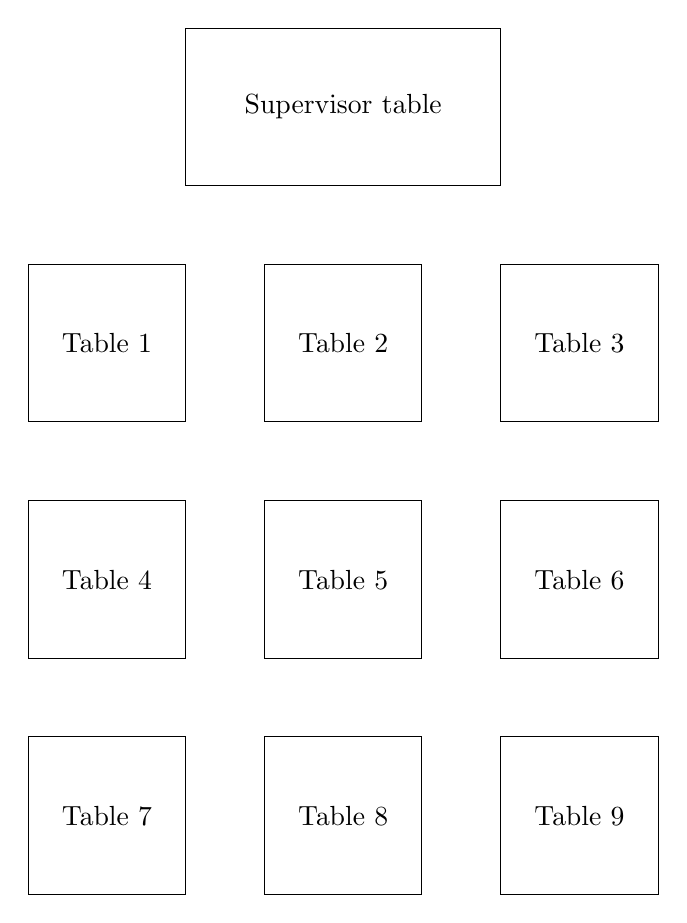
\begin{tikzpicture}
     		\draw (0,0) rectangle (2,2);\node at (1,1) {Table 7};
     		\draw (3,0) rectangle (5,2);\node at (4,1) {Table 8};
     		\draw (6,0) rectangle (8,2);\node at (7,1) {Table 9};
     		\draw (0,3) rectangle (2,5);\node at (1,4) {Table 4};
     		\draw (3,3) rectangle (5,5);\node at (4,4) {Table 5};
     		\draw (6,3) rectangle (8,5);\node at (7,4) {Table 6};
     		\draw (0,6) rectangle (2,8);\node at (1,7) {Table 1};
     		\draw (3,6) rectangle (5,8);\node at (4,7) {Table 2};
     		\draw (6,6) rectangle (8,8);\node at (7,7) {Table 3};
     		\draw (2,9) rectangle (6,11);\node at (4,10) {Supervisor table};
		\end{tikzpicture}
		}
\end{document}
